\documentclass[a4paper,11pt]{article}
\usepackage{amsmath}
\usepackage{amssymb}
\usepackage[polish]{babel}
\usepackage{polski}
\usepackage[utf8]{inputenc}
\usepackage{indentfirst}
\usepackage{geometry}
\usepackage{array}
\usepackage[pdftex]{color,graphicx}
\usepackage{subfigure}
\usepackage{afterpage}
\usepackage{setspace}
\usepackage{color}
\usepackage{wrapfig}
\usepackage{listings}
\usepackage{datetime}

\renewcommand{\onehalfspacing}{\setstretch{1.6}}

\geometry{tmargin=2.5cm,bmargin=2.5cm,lmargin=2.5cm,rmargin=2.5cm}
\setlength{\parindent}{1cm}
\setlength{\parskip}{0mm}

\newenvironment{lista}{
\begin{itemize}
  \setlength{\itemsep}{1pt}
  \setlength{\parskip}{0pt}
  \setlength{\parsep}{0pt}
}{\end{itemize}}

\newcommand{\linia}{\rule{\linewidth}{0.4mm}}

\definecolor{lbcolor}{rgb}{0.95,0.95,0.95}
\lstset{
    backgroundcolor=\color{lbcolor},
    tabsize=4,
  language=C++,
  captionpos=b,
  tabsize=3,
  frame=lines,
  numbers=left,
  numberstyle=\tiny,
  numbersep=5pt,
  breaklines=true,
  showstringspaces=false,
  basicstyle=\footnotesize,
  identifierstyle=\color{magenta},
  keywordstyle=\color[rgb]{0,0,1},
  commentstyle=\color{Darkgreen},
  stringstyle=\color{red}
  }

\begin{document}

\noindent
\begin{tabular}{|c|p{11cm}|c|} \hline 
Z2 & Przemysław Kleszcz, Krzysztof Tatar & \ddmmyyyydate\today \tabularnewline
\hline 
\end{tabular}


\section*{Zadanie 5 - Liczby pierwsze - MPI}

Celem zadania było napisanie programu, który testuje podane duże liczby pierwsze. Do poprawnego działania programu należy podać dwa argumenty wejściowe są to \emph{n -liczba procesów} i \emph{primes - ścieżka do pliku z liczbami pierwszym}. Poniżej zaprezentowano główną funkcje programu odpowiedzialną za zrównoleglanie obliczeń.


\begin{lstlisting}
	MPI_Init(NULL, NULL);
	MPI_Comm_size(MPI_COMM_WORLD, &world_size);
	MPI_Comm_rank(MPI_COMM_WORLD, &world_rank);
int prime_number(string tnumber)
{
	int prime = 1;
	long long j;
	long long number = atoll(tnumber.c_str());
	long long sqrtNumber = sqrtl(number);
	bool flag = false;
	for (j = 2; j < sqrtNumber; j++)
	{
		if (flag)
			continue;
		if (number % j == 0)
		{
			prime = 0;
			flag = true;
		}
	}
	return prime;
}
		MPI_Recv(&k, 1, MPI_INT, 0, 0, MPI_COMM_WORLD, MPI_STATUS_IGNORE);
		MPI_Recv(tableOfRes, k, MPI_LONG_LONG, 0, 0, MPI_COMM_WORLD, MPI_STATUS_IGNORE);
		MPI_Send(&k, 1, MPI_INT, 0, 0, MPI_COMM_WORLD);
		MPI_Send(tableOfRes, k, MPI_LONG_LONG, 0, 0, MPI_COMM_WORLD);
		MPI_Send(tableOfResb, k, MPI_INT, 0, 0, MPI_COMM_WORLD);
\end{lstlisting}

Powyższy program sprawdza czy liczba jest pierwszą czy nie jest liczbą pierwszą. Do zrównoleglenia głównej pętli for została użyta biblioteka MPI.

Funkcje MPI użyte w programie.
\begin{lstlisting}
MPI_Init(argc, argv);
\end{lstlisting}
Funkcja inicjalizuje środowisko wykonywania programu, m.in. tworzy domyślny komunikator \newline MPI\_COMM\_WORLD. Dopiero od momentu wywołania MPI\_Init można używać pozostałych funkcji MPI
\begin{lstlisting}
MPI_Comm_rank(MPI_COMM_WORLD, numberOfProcess);
\end{lstlisting}
Funkcja pobiera numer aktualnego procesu (w obrębie komunikatora comm) i umieszcza go w zmiennej rank.
\begin{lstlisting}
MPI_Comm_size(MPI_COMM_WORLD, processes);
\end{lstlisting}
Funkcja pobiera ilość procesów (w obrębie komunikatora comm i umieszcza ją w zmiennej size.
\begin{lstlisting}
MPI_Finalize()
\end{lstlisting}
Funkcja zwalnia zasoby używane przez MPI i przygotowuje system do zamknięcia.

\begin{lstlisting}
MPI_Recv(data, size, type, destination, tag, communicator, MPI_STATUS_IGNORE);
\end{lstlisting}
Funkcja odczytuje z kolejki komunikatora communicator (z ewentualnym blokowaniem do czasu nadejścia) pierwszy komunikat od procesu source oznaczony znacznikiem tag typu datatype. Wynik umieszczany jest w buforze data a status operacji w zmiennej status.

\begin{lstlisting}
 MPI_Send(dane, rozmiar, typ, destination, tag, communicator);
\end{lstlisting}
Funkcja wysyła komunikat typu datatype do procesu numer dest oznaczony znacznikiem tag w obrębie komunikatora communicator.
Typ komunikatu jest zawarty w zmiennej datatype i może to być któryś z predefiniowanych typów np.  MPI\_INT lub inne. Tag jest liczbą w zakresie [0..MPI\_TAG\_UB] i określa dodatkowy typ komunikatu wykorzystywany przy selektywnym odbiorze funkcją MPI\_Recv.


\begin{figure}[!ht]
	\centering
 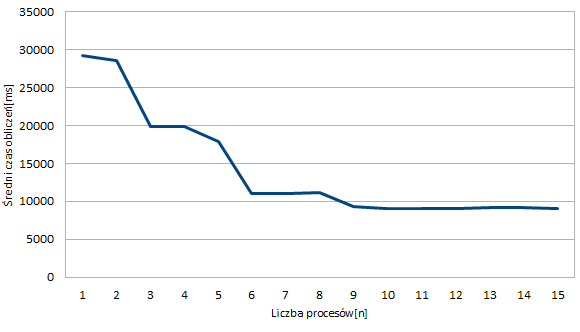
\includegraphics[width=0.7\textwidth]{1.png}
  \caption{Wykres średniego czasu obliczeń}
\end{figure}

Z powyższego rysunku można wywnioskować, że średni czas obliczeń dynamicznie przyspieszył dla pierwszych 3 procesów. Następnie od 3 do 4 procesu czas jest równomierny. Kolejny znaczy skok w przyspieszeniu jest od 4 do 6 procesu. Następnie średni czas jest stały.
Poniższy rysunek jest dobrym przykładem opisanego zjawiska.

\begin{figure}[ht]
	\centering
  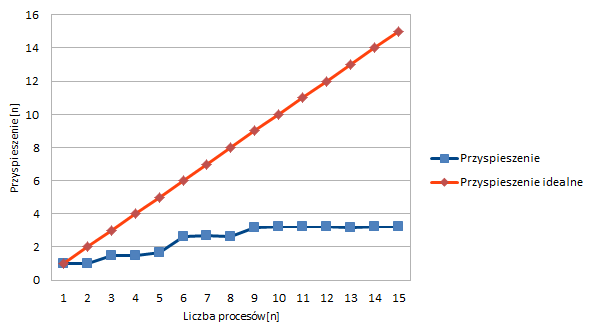
\includegraphics[width=0.7\textwidth]{2.png}
  \caption{Wykres przyspieszenia}
\end{figure}

Powyższe zadanie zostało zrównoleglone dzięki bibliotece MPI (Message Passing Interface). Udało się uzyskać prawie czterokrotne przyspieszenie dla 9 procesów. Dla kolejnych  procesów, w tym przykładzie nie wpłynęły znacząco na wydajność, wykres ma postać stałej.
\end{document}
